% interactcadsample.tex
% v1.03 - April 2017

\documentclass[]{interact}

\usepackage{epstopdf}% To incorporate .eps illustrations using PDFLaTeX, etc.
\usepackage{subfigure}% Support for small, `sub' figures and tables
%\usepackage[nolists,tablesfirst]{endfloat}% To `separate' figures and tables from text if required

\usepackage{natbib}% Citation support using natbib.sty
\bibpunct[, ]{(}{)}{;}{a}{}{,}% Citation support using natbib.sty
\renewcommand\bibfont{\fontsize{10}{12}\selectfont}% Bibliography support using natbib.sty

\theoremstyle{plain}% Theorem-like structures provided by amsthm.sty
\newtheorem{theorem}{Theorem}[section]
\newtheorem{lemma}[theorem]{Lemma}
\newtheorem{corollary}[theorem]{Corollary}
\newtheorem{proposition}[theorem]{Proposition}

\theoremstyle{definition}
\newtheorem{definition}[theorem]{Definition}
\newtheorem{example}[theorem]{Example}

\theoremstyle{remark}
\newtheorem{remark}{Remark}
\newtheorem{notation}{Notation}

% see https://stackoverflow.com/a/47122900
\usepackage{color}
\usepackage{fancyvrb}
\newcommand{\VerbBar}{|}
\newcommand{\VERB}{\Verb[commandchars=\\\{\}]}
\DefineVerbatimEnvironment{Highlighting}{Verbatim}{commandchars=\\\{\}}
% Add ',fontsize=\small' for more characters per line
\usepackage{framed}
\definecolor{shadecolor}{RGB}{248,248,248}
\newenvironment{Shaded}{\begin{snugshade}}{\end{snugshade}}
\newcommand{\AlertTok}[1]{\textcolor[rgb]{0.94,0.16,0.16}{#1}}
\newcommand{\AnnotationTok}[1]{\textcolor[rgb]{0.56,0.35,0.01}{\textbf{\textit{#1}}}}
\newcommand{\AttributeTok}[1]{\textcolor[rgb]{0.77,0.63,0.00}{#1}}
\newcommand{\BaseNTok}[1]{\textcolor[rgb]{0.00,0.00,0.81}{#1}}
\newcommand{\BuiltInTok}[1]{#1}
\newcommand{\CharTok}[1]{\textcolor[rgb]{0.31,0.60,0.02}{#1}}
\newcommand{\CommentTok}[1]{\textcolor[rgb]{0.56,0.35,0.01}{\textit{#1}}}
\newcommand{\CommentVarTok}[1]{\textcolor[rgb]{0.56,0.35,0.01}{\textbf{\textit{#1}}}}
\newcommand{\ConstantTok}[1]{\textcolor[rgb]{0.00,0.00,0.00}{#1}}
\newcommand{\ControlFlowTok}[1]{\textcolor[rgb]{0.13,0.29,0.53}{\textbf{#1}}}
\newcommand{\DataTypeTok}[1]{\textcolor[rgb]{0.13,0.29,0.53}{#1}}
\newcommand{\DecValTok}[1]{\textcolor[rgb]{0.00,0.00,0.81}{#1}}
\newcommand{\DocumentationTok}[1]{\textcolor[rgb]{0.56,0.35,0.01}{\textbf{\textit{#1}}}}
\newcommand{\ErrorTok}[1]{\textcolor[rgb]{0.64,0.00,0.00}{\textbf{#1}}}
\newcommand{\ExtensionTok}[1]{#1}
\newcommand{\FloatTok}[1]{\textcolor[rgb]{0.00,0.00,0.81}{#1}}
\newcommand{\FunctionTok}[1]{\textcolor[rgb]{0.00,0.00,0.00}{#1}}
\newcommand{\ImportTok}[1]{#1}
\newcommand{\InformationTok}[1]{\textcolor[rgb]{0.56,0.35,0.01}{\textbf{\textit{#1}}}}
\newcommand{\KeywordTok}[1]{\textcolor[rgb]{0.13,0.29,0.53}{\textbf{#1}}}
\newcommand{\NormalTok}[1]{#1}
\newcommand{\OperatorTok}[1]{\textcolor[rgb]{0.81,0.36,0.00}{\textbf{#1}}}
\newcommand{\OtherTok}[1]{\textcolor[rgb]{0.56,0.35,0.01}{#1}}
\newcommand{\PreprocessorTok}[1]{\textcolor[rgb]{0.56,0.35,0.01}{\textit{#1}}}
\newcommand{\RegionMarkerTok}[1]{#1}
\newcommand{\SpecialCharTok}[1]{\textcolor[rgb]{0.00,0.00,0.00}{#1}}
\newcommand{\SpecialStringTok}[1]{\textcolor[rgb]{0.31,0.60,0.02}{#1}}
\newcommand{\StringTok}[1]{\textcolor[rgb]{0.31,0.60,0.02}{#1}}
\newcommand{\VariableTok}[1]{\textcolor[rgb]{0.00,0.00,0.00}{#1}}
\newcommand{\VerbatimStringTok}[1]{\textcolor[rgb]{0.31,0.60,0.02}{#1}}
\newcommand{\WarningTok}[1]{\textcolor[rgb]{0.56,0.35,0.01}{\textbf{\textit{#1}}}}

% Pandoc citation processing

\usepackage{hyperref}
\usepackage[utf8]{inputenc}
\usepackage{booktabs}
\usepackage{bm}
\usepackage{mathtools}
\usepackage{amssymb}
\usepackage{amsmath}
\usepackage{tikz}
\usetikzlibrary{arrows}
\usepackage[nofiglist]{endfloat}
\usepackage{blkarray}
\usepackage{setspace}
\usepackage{etoolbox}
\DeclareMathOperator{\E}{\mathbb{E}}
\DeclareMathOperator{\Var}{\mathrm{Var}}
\DeclareMathOperator{\Cov}{\mathrm{Cov}}
\DeclareMathOperator*{\argmax}{arg\,max}
\DeclareMathOperator*{\argmin}{arg\,min}
\mathtoolsset{showonlyrefs}
\BeforeBeginEnvironment{equation}{\begin{singlespace}\vspace*{-\baselineskip}}
\AfterEndEnvironment{equation}{\end{singlespace}\noindent\ignorespaces}
\BeforeBeginEnvironment{align}{\begin{singlespace}\vspace*{-\baselineskip}}
\AfterEndEnvironment{align}{\end{singlespace}\noindent\ignorespaces}
\def\tightlist{}
\pagenumbering{gobble}


\begin{document}

\articletype{TEACHER'S CORNER}

\title{A closer look at random and fixed effects panel regression in
structural equation modeling using \texttt{lavaan}}


\author{\name{Henrik Kenneth Andersen$^{a}$}
\affil{$^{a}$Chemnitz University of Technology, Institute of Sociology,
Chair for Empirical Social Research, Thüringer Weg 9, 09126 Chemnitz,
Germany}
}

\thanks{CONTACT Henrik Kenneth
Andersen. Email: \href{mailto:henrik.andersen@soziologie.tu-chemnitz.de}{\nolinkurl{henrik.andersen@soziologie.tu-chemnitz.de}}}

\maketitle

\begin{abstract}
This article provides an in-depth look at random and fixed effects panel
regression in the structural equation modeling (SEM) framework,
specifically the application of fixed effects in the \texttt{lavaan}
package for \texttt{R}. It is meant as a applied guide for researchers,
covering the underlying model specification, syntax, and summary output.
\end{abstract}

\begin{keywords}
Fixed effects, structural equation modeling, lavaan, R, panel
regression, longitudinal data
\end{keywords}

\newpage

\pagenumbering{arabic} 
\setcounter{page}{1}

\doublespacing

\hypertarget{intro}{%
\section{Introduction}\label{intro}}

Several years ago, \citet{Curran2011} reflected positively on the
growing use of panel studies in empirical social research. Some of the
strengths of panel data are well-known, e.g., the ability to establish
temporal precedence, increased statistical power and the reduction of
potential alternative models. However, perhaps the greatest strength of
panel data is that they allow for a more rigorous testing of substantive
theories. Panel data, i.e., repeated measures of the same observed units
(people, schools, firms, countries, etc.), allow researchers to
decompose the error term into a part that stays constant within units
and the part that changes over time. The part that does not change over
time can be seen as the combined effect of all time-invariant influences
(e.g., sex, date of birth, nationality) on the dependent variable.
Random effects (RE) and fixed effects (FE) regression involve accounting
for these often unobserved time-invariant influences via a number of
methods. In the case of RE models, it is assumed that the stable
characteristics are unrelated to the other model covariates. In that
case, the stable characteristics, or individual effects as they are
often referred to as, will not affect point estimates but are a source
of error variance that, if ignored, lead to larger standard errors and
increase the likelihood of type II errors (failure to reject a false
null hypothesis). FE models are useful when the individual effects are
expected to be related to one or more of the model covariates. In that
case, these unobserved stable characteristics will act as confounders
and lead to biased point estimates. In controlling for these individual
effects, FE regression thus accounts for a likely and common source of
bias.

Structural equation modeling (SEM) is a popular regression framework.
One of its main strengths is its flexibility. Not only can complex
causal structures with multiple dependent variables be tested
simultaneously, but in longitudinal (and, more generally, hierarchical)
studies both time-varying and invariant predictors can be included, and
effects can easily be allowed to vary over time. Thus researchers can
allow for and study effects that increase or fade over time, or that
appear only in specific periods. Beyond that, with the use of latent
variables, SEM provides a way to deal with measurement error and get
closer to the theoretical constructs of interest.

There are a number of articles describing basic concept of panel model
regression, including RE and FE regression in SEM
\citep[e.g.,][]{Allison2011, Bollen2010, Teachman2001}. This article is
intended as a \textit{practical guide} for researchers looking for help
specifying panel regression models in SEM. It assumes some basic
knowledge of SEM (i.e., minimizing the difference between observed and
model-implied covariance matrices and mean vectors, maximum likelihood
estimation, etc.);\footnote{For an introduction to SEM,
  \citet{Bollen1989} is a classic for good reason, and
  \citet{Ferron2007} lay out exactly how SEM works in one easy to follow
  article.} perhaps the reader is an experienced SEM-user looking for a
quick guide to estimating the static panel models discussed here; or,
perhaps the reader is new to SEM, potentially because an adviser or
superior has suggested it to them. For the latter case, this article
reviews the assumptions associated with the more tradititonal least
squares-based approach to RE and FE models, so that the implementation
in SEM is more easily to follow. The article focuses on the
\texttt{lavaan} \citep{R-lavaan} package for \texttt{R} \citep{R-base}.
While \texttt{Mplus} \citep{Mplus} is arguably the most robust SEM
software currently available (in terms of features like alignment,
latent variable interactions, for example), the \texttt{lavaan} package
has many benefits. First, like \texttt{R} it is open source and
completely free. For researchers dipping their toes into SEM, there is
no financial barrier to try, and no risk if they decide it is not for
them. Second, the implementation of \texttt{lavaan} in the larger
\texttt{R} environment is an enormous advantage. Instead of poring over
reams of plain text, copying out coefficients by hand, every part of the
\texttt{lavaan} output is available as an object. This means that all
aspects of the model, from fit indices, to coefficients and standard
errors, to the model matrices, can be accessed and easily integrated
into tables and plots. Furthermore, \texttt{R} can be used for a great
deal of applications. It can be used to manage and manipulate as well as
simulate data, perform symbolic algebra, run more traditional analyses
(e.g., multiple regression, logistic regression, principal component
analysis), etc. Once one is comfortable using \texttt{R}, there is no
longer any need to switch between different software for data
preparation and analysis.

The following article outlines the basic idea of panel regression, the
particularities of panel regression SEM, and shows its implementation in
\texttt{lavaan}. Using
\href{https://github.com/henrik-andersen/FE-SEM/blob/master/simulation-code.R}{simulated
data}, it demonstrates and annotates the code for the most basic FE
model and provides an overview of the summary output. One of the main
strengths of panel SEM compared to the more traditional methods of panel
analysis is its flexibility. Therefore, a number of potential extensions
to the basic model, including relaxing various assumptions, dealing with
measurement error in both the independent and dependent variables, as
well as the inclusion of time-invariant predictors in the form of a
hybrid fixed-/ random effects model, are shown in detail in the form of
\href{https://github.com/henrik-andersen/FE-SEM/blob/master/extensions.pdf}{online
supplementary materials}.

\hypertarget{panel}{%
\section{Random and Fixed Effects Panel models}\label{panel}}

It is typically the case that the values for a given unit on a variable
at one point in time will tend to tell us something about that unit's
values at another point in time. There are two main explanations for
this `empirical regularity'
\citetext{\citealp{Heckman1981}; \citealp[p.~261]{Hsiao2014}; \citealp{Bruederl2015}; \citealp{Bianconcini2018}}.
First, it could be that an experience at one point in time has a
causal\footnote{Here the word causal is used to mean `non-spurious'.}
effect on future experiences. In other words, experiencing an event
could change the probability of the same or a similar event taking place
in the future. For example, if employment increases wages, then the
incentive to continue working should increase over time, thereby making
it more likely that someone who was employed at one point in time will
continue to be employed in the future \citep{Heckman1981}. When past
experiences causally impact future events, the empirical regularity is
referred to as `state dependence'. So-called `dynamic' panel models that
include the lagged dependent variable in the equation for the current
dependent variable, like autoregressive and autoregressive cross-lagged
models, are examples of panel models that account for state dependence.
The second explanation is that correlations over time are due to stable
unobservables, like sex, place of birth, motivation, ability or
personality characteristics.\footnote{From here on out the units of
  interest are assumed to be individuals, but other units of observation
  like schools, companies, countries, etc., are possible.} In other
words, stable unit-specific characteristics might predispose individuals
to experiencing events with a certain likelihood over time. For example,
stable characteristics like an individual's sex and motivation could be
part of the reason why some individuals tend to be continuously
employed, while others experience spells of unemployment, or are
habitually unemployed. This second source of empirical regularity is
referred to as individual heterogeneity or, more generally, unobserved
heterogeneity \citep{Wooldridge2012}. So-called `static' panel models
(that do not include the lagged dependent variable in the equation for
the current one) focus on this second source of empirical regularity.

The random and fixed effects models that will be discussed here are
examples of models that attempt to account for unobserved heterogeneity
as a source of empirical regularity. In the case of both the random and
fixed effects models, it is assumed that there exist stable individual
characteristics that affect the dependent variable of interest over
time. Failure to account for this source of stable variance will reduce
model fit. If any of the stable characteristics are related to the model
covariates (a plausible scenario in many cases where the independent
variable(s) of interest are not fixed), then they must also be
considered confounders, and failure to account for them will further
lead to biased point estimates.\footnote{Whether or not the stable
  individual characteristics are related to the model covariates is the
  modern differentiator between random effects, where the individual
  effects are assumed independent of the covariates, and fixed effects,
  where the individual effects are assumed to be related to one or more
  of them, see \citet{Wooldridge2012}, p.~251. This can be a cause for
  confusion for those who are more familiar with the mixed or multilevel
  model framework. There, `fixed' effects are those coefficients that
  apply to the entire sample, `random' effects are the variance
  components for the higher level grouping variables, see for example
  \citet{Hox2010}; \citet{Bates2015}; \citet{R-lme4}.}

In this section, the basic random and fixed effects models, as well as
their implementation in SEM, will be discussed. Later on in the article,
it will be discussed how to extend the model, by relaxing some
assumptions and introducing other time-invariant predictors in a type of
`hybrid' random and fixed effects model. The outlook will describe
further extensions, such as the inclusion of lagged dependent variable
for a dynamic panel model with individual effects.\\
Let us begin with a simple linear `unobserved effects model'
\citep{Wooldridge2012, R-plm_a} \begin{align}
y_{it} & = \beta_{0} + \beta_{1} x_{it} + \alpha_{i} + \varepsilon_{it}, \ i = 1, \ldots, N, \ t = 1, \ldots, T \label{eq:panel-model}
\end{align} where \(y_{it}\) is the dependent variable for unit \(i\) at
time \(t\) and \(x_{it}\) is a single covariate with associated scalar
coefficient \(\beta_{1}\). \(\alpha_{i}\) represents the combined effect
of all unobserved time-constant variables affecting the dependent
variable and \(\varepsilon_{it}\) is the idiosyncratic error. This model
could of course be extended by turning \(x_{it}\) into a vector of
covariates
\(\bm{x}_{it} = (x_{1_{it}}, x_{2_{it}}, \ldots, x_{k_{it}})\), or by
introducing time-invariant covariates,
\(\bm{z}_{i} = (z_{1_{i}}, z_{2_{i}}, \ldots, z_{m_{i}})\), but we want
to first focus on assumptions and mechanics before moving on to
discussing possibilities for extending the model.

Equation \eqref{eq:panel-model} is often written in matrix form for unit
\(i\) as \begin{align}
\bm{y}_{i} & = \bm{\iota}_{T}\beta_{0} + \bm{x}_{i}\beta_{1} + \bm{\iota}_{T} \alpha_{i} + \bm{\varepsilon}_{i}, \ i = 1, \ldots, N \label{eq:matrix-panel-model}
\end{align} where
\(\bm{y}_{i} = (y_{i1}, y_{i2}, \ldots, y_{iT})^{\intercal}\) and
\(\bm{x}_{i} = (x_{i1}, x_{i2}, \ldots, x_{iT})^{\intercal}\) are
\(T \times 1\) vectors of each of the \(t\) observations for unit \(i\),
\(\bm{\iota}_{T}\) is a \(T \times 1\) vector of ones and
\(\bm{\varepsilon}_{i} = (\varepsilon_{i1}, \varepsilon_{i2}, \ldots, \varepsilon_{iT})^{\intercal}\)
is likewise a \(T \times 1\) vector of errors. It may be helpful to keep
this Equation \eqref{eq:matrix-panel-model} in mind later when we
restate the model for estimation using SEM. There, we will take the
long-format data and transform it into wide-format.

\hypertarget{assumptions-in-least-squares-based-approaches}{%
\subsection{Assumptions in least squares-based
approaches}\label{assumptions-in-least-squares-based-approaches}}

One of the main strengths of SEM is the flexibility it affords. Nearly
every part of the model is specified `by hand', so to speak (although
modern SEM software has come a long way from, say, \texttt{EQS}
\citep{Bentler2006}, where the errors and disturbances had to be
mentioned in the syntax and now comes with a variety of default settings
for ease of use), which means model assumptions are conveyed directly,
by the user specifying paths and correlations and setting other
relations to zero. Common least squares-based statistical packages
\citep[like the \texttt{plm} package in \texttt{R},][]{R-plm_a} require
less input from the user (usually it is enough to input the model
variables and specify some top-level options). The assumptions in the
least squares-based models are widely known
\citep{Wooldridge2012, Bruederl2015, Greene2012, Angrist2009} but do not
come into play prominently while specifying the model. So here we will
discuss the `typical' assumptions associated with least squares-based
random and fixed effects models. Later, when we examine the
implementation in SEM, we will then be able to relate back to this
discussion.\footnote{What constitutes a `typical' least squares-based
  approach to these panel regression models is likely debatable. Here,
  this refers broadly to the assumptions discussed in the literature and
  default settings one encounters in statistical packages intended for
  this purpose.}

We want to relate the SEM-based approach to random and fixed effects to
the least squares-based approach which is likely more widely known and
more straightforward to implement, i.e., statistical packages for static
panel regression models exist (e.g., the \texttt{plm} package in
\texttt{R}, see \citet{R-plm_a}), and typically only require the user to
enter the model variables and specify some top-level options (random
effects vs.~fixed effects, individual vs.~individual and time effects,
etc.). The model assumptions for random and fixed effects models are
widely known
\citep{Wooldridge2012, Bruederl2015, Greene2012, Angrist2009} but are
not prominent in th

The least squares-based approach to such a panel model typically makes
the following base assumptions:\footnote{What constitutes a `typical'
  least squares-based approach to these panel regression models is
  likely debatable. Here, this refers broadly to the default assumptions
  and settings one encounters in statistical packages intended for this
  purpose, like the \texttt{plm} package in \texttt{R}, see
  \citet{R-plm_a}.} first, the mean function is linear, i.e.,
\(\mathop{\mathrm{\mathbb{E}}}(y_{it} | x_{it}, \alpha_{i}) = \beta_{0} + \beta_{1} x_{it} + \alpha_{i}\),
and second, that the cross-sectional observations are independent, which
is assured by random sampling \citep{Wooldridge2012}. Further, and just
as with any other regression model, the idiosyncratic error is assumed
to be mean independent of the model covariates and the individual
effects, i.e.,
\(\mathop{\mathrm{\mathbb{E}}}(\varepsilon_{it} | x_{it}, \alpha_{i}) = \mathop{\mathrm{\mathbb{E}}}(\varepsilon_{it}) = 0\).\footnote{If
  there is an overall intercept, \(\beta_{0}\), then it is safe to
  assume the unconditional expectation of the idiosyncratic error is
  zero, i.e., \(\mathop{\mathrm{\mathbb{E}}}(\varepsilon_{it}) = 0\).}
The mean independence assumption also implies the assumption of a zero
correlation between the idiosyncratic error and the model covariates,
i.e., \(\mathop{\mathrm{\mathbb{E}}}(x_{it}\varepsilon_{it}) = 0\).

The (modern) difference between random and fixed effects boils down to
the assumption of the relatedness of the model covariates and the
individual effects. The random effects model assumes the model
covariates are unrelated to the individual effects, i.e., in this case
\(\mathop{\mathrm{\mathbb{E}}}(\alpha_{i} | x_{it}) = \mathop{\mathrm{\mathbb{E}}}(\alpha_{i})\)
and thus \(\mathop{\mathrm{\mathbb{E}}}(\alpha_{i}x_{it}) = 0\). As
such, we could put \(\alpha_{i}\) into the error term to form the
composite error, \(\nu_{it} = \alpha_{i} + \varepsilon_{it}\), and the
point estimates of the coefficients of interest, here \(\beta_{1}\),
would be consistent (assuming the model is otherwise correctly
specified). The problem with putting the individual effects into the
error term is that it would induce dependency between the compostie
errors within the same individual, which goes against the independence
assumption \citep{Wooldridge2012, Schmidheiny2019}. We will discuss that
in more detail below. In the fixed effects model, one or more of the
model covariates are assumed to be related to the individual effects,
here
\(\mathop{\mathrm{\mathbb{E}}}(\alpha_{i} | x_{it}) \ne \mathop{\mathrm{\mathbb{E}}}(\alpha_{i})\)
and thus \(\mathop{\mathrm{\mathbb{E}}}(\alpha_{i}x_{it}) \ne 0\). Thus,
ignoring the individual heterogeneity and putting \(\alpha_{i}\) into
the error term would mean that point estimates of the coefficients of
interest would be inconsistent.

The traditional least squares-based approaches to random and fixed
effects often assume as well that the errors are homoskedastictic over
time, i.e.,
\(\mathop{\mathrm{\mathbb{E}}}(\varepsilon_{it}^{2}) = \sigma_{\varepsilon_{t}}^{2} = \sigma_{\varepsilon}^{2}\).
The individual effects are assumed to have a constant partial effect on
the dependent variable over time \citep[p.~248]{Wooldridge2012}. Also,
typically least squares-based approaches stack each of the \(N\)
repeated measures per individual \(i\) and calculate one single
coefficient per variable for the entire sample. I.e., it is generally
not intended that the estimated coefficient should vary across \(t\) or
\(i\).

\hypertarget{random-and-fixed-effects-in-sem}{%
\section{Random and fixed effects in
SEM}\label{random-and-fixed-effects-in-sem}}

For panel regression in SEM, we typically convert any stacked,
long-format vectors of observations of length \(NT\) into \(T\) separate
vectors of length \(N\). In doing so, we get \(T\) individual equations
for each time point \begin{align}
\bm{y}_{t} & = \bm{\iota}_{N}\beta_{0_{t}} + \bm{x}_{t}\beta_{1_{t}} + \bm{\alpha} + \bm{\varepsilon}_{t}, \ t = 1, \ldots, T \\
\begin{bmatrix}
y_{1_{t}} \\
y_{2_{t}} \\
\vdots \\
y_{N_{t}}
\end{bmatrix} & = 
\begin{bmatrix}
1 \\
1 \\ 
\vdots \\
1
\end{bmatrix} \beta_{0_{t}} + 
\begin{bmatrix}
x_{1_{t}} \\
x_{2_{t}} \\
\vdots \\
x_{N_{t}}
\end{bmatrix} \beta_{1_{t}} + 
\begin{bmatrix}
\alpha_{1} \\
\alpha_{2} \\
\vdots \\
\alpha_{N}
\end{bmatrix} + 
\begin{bmatrix}
\varepsilon_{1_{t}} \\
\varepsilon_{2_{t}} \\
\vdots \\
\varepsilon_{N_{t}}
\end{bmatrix}
\end{align}

Let us discuss the random and fixed effects models in SEM by examining a
path diagram. Figure \ref{fig:panel-sem} shows a four-wave panel model
with individual effects. As usual, rectangles indicate observed
variables and circles indicate latent variables. One-sided errors
indicate effects and two-headed errors indicate correlations or
covariances.

We assume all of the observed variables are grand mean centered, so that
we can drop the overall intercept from the model.

\begin{figure}
\begin{center}
\resizebox{0.75\textwidth}{!}{%
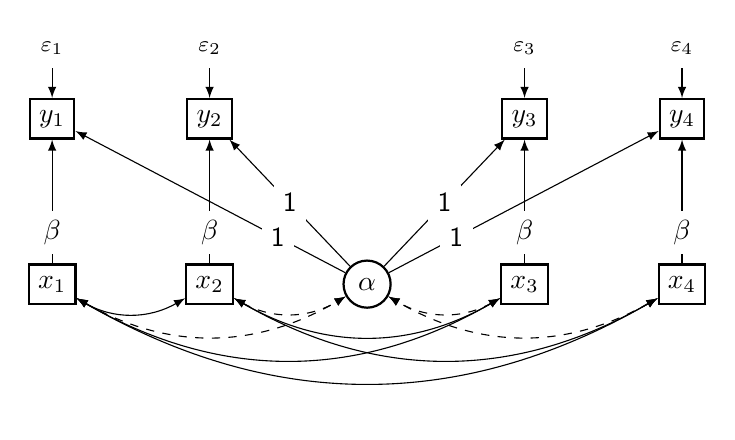
\begin{tikzpicture}
% Node styles ---
\tikzstyle{man} = [rectangle, thick, minimum size = 0.5cm, draw = black!100, fill = white!100, font = \sffamily] 
\tikzstyle{lat} = [circle, thick, minimum size = 0.5cm, draw = black!100, fill = white!100, font = \sffamily] 
\tikzstyle{err} = [rectangle, minimum size = 0.5cm, draw = white!100, fill = white!100, font = \sffamily] 
\tikzstyle{pha} = [rectangle, minimum size = 0.001cm, draw = white, fill = white]
\tikzstyle{con} = [-latex, draw = black!100, font = \sffamily] 
\tikzstyle{seqex} = [latex-latex, draw = black!100, font = \sffamily, dashed]
\tikzstyle{cons} = [-latex, draw = black!100, font = \sffamily\small] 
\tikzstyle{cor} = [latex-latex, font = \sffamily] 
% Begin Figure ---
% Nodes 
\node at (+0.0,+0.0) [man] (x1) {$x_{1}$};
\node at (+2.0,+0.0) [man] (x2) {$x_{2}$};
\node at (+6.0,+0.0) [man] (x3) {$x_{3}$};
\node at (+8.0,+0.0) [man] (x4) {$x_{4}$};
\node at (+4.0,+0.0) [lat] (alp) {$\alpha$};
\node at (+0.0,+2.1) [man] (y1) {$y_{1}$};
\node at (+2.0,+2.1) [man] (y2) {$y_{2}$};
\node at (+6.0,+2.1) [man] (y3) {$y_{3}$};
\node at (+8.0,+2.1) [man] (y4) {$y_{4}$};
\node at (+0.0,+3.0) [err] (e1) {\footnotesize $\varepsilon_{1}$};
\node at (+2.0,+3.0) [err] (e2) {\footnotesize $\varepsilon_{2}$};
\node at (+6.0,+3.0) [err] (e3) {\footnotesize $\varepsilon_{3}$};
\node at (+8.0,+3.0) [err] (e4) {\footnotesize $\varepsilon_{4}$};
% Paths
\path (alp) edge [con] node [near start, fill=white] {1} (y1);
\path (alp) edge [con] node [midway, fill=white] {1} (y2);
\path (alp) edge [con] node [midway, fill=white] {1} (y3);
\path (alp) edge [con] node [near start, fill=white] {1} (y4);
\path (x1) edge [con] node [near start, fill=white] {$\beta$} (y1);
\path (x2) edge [con] node [near start, fill=white] {$\beta$} (y2);
\path (x3) edge [con] node [near start, fill=white] {$\beta$} (y3);
\path (x4) edge [con] node [near start, fill=white] {$\beta$} (y4);
\path (e1) edge [con] node {} (y1);
\path (e2) edge [con] node {} (y2);
\path (e3) edge [con] node {} (y3);
\path (e4) edge [con] node {} (y4);
% correlations
\path (x1) edge [cor, bend right] node {} (x2);
\path (x1) edge [seqex, bend right] node {} (alp);
\path (x1) edge [cor, bend right] node {} (x3);
\path (x1) edge [cor, bend right] node {} (x4);
\path (x2) edge [seqex, bend right] node {} (alp);
\path (x2) edge [cor, bend right] node {} (x3);
\path (x2) edge [cor, bend right] node {} (x4);
\path (x3) edge [seqex, bend left] node {} (alp);
\path (x4) edge [seqex, bend left] node {} (alp); 
\end{tikzpicture}
}
\caption{Four-wave static panel model\label{fig:panel-sem}}
\end{center}
\end{figure}

To begin, let us review a general panel model \citep{Bollen2010}, also
referred to as the `unobserved effects model'
\citep{Wooldridge2012, R-plm_a} (we will return to this model in the
\href{https://github.com/henrik-andersen/FE-SEM/blob/master/extensions.pdf}{online
supplementary materials} when we discuss loosening assumptions)
\begin{align}
y_{it} & = \bm{x}_{it}\bm{\beta} + \bm{z}_{i}\bm{\gamma} + \alpha_{i} + \varepsilon_{it} \label{eq:gpm}
\end{align} where \(y_{it}\) is the dependent variable for unit
\(i, \ i = 1, ..., N\) at time \(t, \ t = 1, ..., T\), \(\bm{x}_{it}\)
is a \(1 \times K\) vector of time-varying covariates (which could
include a constant) linked to the dependent variable by the
\(K \times 1\) vector of coefficients \(\bm{\beta}\). \(\bm{z}_{i}\) is
a \(1 \times M\) vector of time-invariant covariates linked to the
dependent variable by the \(M \times 1\) vector of coefficients in
\(\bm{\gamma}\), \(\alpha_{i}\) represents the combined effect of all
unobserved time-constant variables affecting the dependent variable and
\(\varepsilon_{it}\) is the idiosyncratic error.

We can make stating some of the model assumptions easier by rewriting it
in matrix notation \begin{align}
\bm{y}_{i} & = \bm{X}_{i}\bm{\beta} + \bm{Z}_{i}\bm{\gamma} + \bm{\iota}_{T}\alpha_{i} + \bm{\varepsilon}_{i}
\end{align} where \(\bm{y}_{i}\) and \(\bm{\varepsilon}_{i}\) are
\(T \times 1\) vectors, \(\bm{X}_{i}\) and \(\bm{Z}_{i}\) are
\(T \times K\) and \(T \times M\) matrices, respectively,
\(\bm{\iota}_{T}\) is a \(T \times 1\) vector of ones and \(\alpha_{i}\)
is a scalar. \(\bm{\beta}\) and \(\bm{\gamma}\) are unchanged from
Equation \eqref{eq:gpm}.

Consistency of the following models requires the assumption of strict
exogeneity, although what constitutes strict exogeneity differs between
the random and fixed effects setups. Each assumption will be discussed
shortly. Apart from that, we typically make the following assumptions
about this model \citep[see, e.g.,][]{Wooldridge2002, Schmidheiny2019}:

\begin{itemize}
\tightlist
\item
  Linearity: the model is linear in its parameters.
\item
  Independence: the observations are independent across individuals
  (assured by random sampling in the cross-section), but not necessarily
  across time.
\item
  The usual rank condition: we have more observations than independent
  variables and there is no perfect collinearity between any of the
  independent variables.
\end{itemize}

\hypertarget{re}{%
\subsection{Random effects}\label{re}}

For the random effects (RE) model, we define a composite error term:
\(\nu_{it} = \alpha_{i} + \varepsilon_{it}\) and rewrite the model in
Equation \eqref{eq:gpm} as \begin{align}
y_{it} & = \bm{x}_{it}\bm{\beta} + \bm{z}_{i}\bm{\gamma} + \nu_{it}, \ \text{or} \\
\bm{y}_{i} & = \bm{X}_{i}\bm{\beta} + \bm{Z}_{i}\bm{\gamma} + \bm{\nu}_{i},
\end{align} where
\(\bm{\nu}_{i} = \alpha_{i} \bm{\iota}_{T} + \bm{\varepsilon}_{i}\) and
\(\bm{\iota}_{T}\) is a \(T \times 1\) vector of ones. The strict
exogeneity assumption in the RE model implies \begin{align}
\mathop{\mathrm{\mathbb{E}}}[\varepsilon_{it} | \bm{X}_{i}, \bm{z}_{i}, \alpha_{i}] & = 0, \\
\mathop{\mathrm{\mathbb{E}}}[\alpha_{i} |\bm{X}_{i}, \bm{z}_{i}] = \mathop{\mathrm{\mathbb{E}}}[\alpha_{i}] & = 0,
\end{align} where \(\bm{X}_{i} = \bm{x}_{i1}, ..., \bm{x}_{iT}\). For
both parts, the assumption that the unconditional expectations are 0 is
unproblematic as long as a constant is included in the regression. The
first part says the idiosyncratic errors at each timepoint are assumed
to be independent of the explanatory variables at \textit{all}
timepoints which is stronger than just assuming that they are
\textit{contemporaneously} independent. This implies that they are also
uncorrelated, i.e.,
\(\mathop{\mathrm{\mathbb{E}}}[\bm{x}_{is}^{\intercal}\varepsilon_{it}] = \bm{0}\)
and
\(\mathop{\mathrm{\mathbb{E}}}[\bm{z}_{i}^{\intercal}\varepsilon_{it}] = \bm{0}, \ \forall \ s, t = 1, ..., T\)
\citep{Wooldridge2002, Bruederl2015}. We assume the idiosyncratic errors
are further independent of the individual effects, which implies
\(\mathop{\mathrm{\mathbb{E}}}[\alpha_{i}\varepsilon_{it}] = 0\).

The second part is the potentially controversial assumption: it states
that the individual effects are uncorrelated with the independent
variables. We can use an intuitive concrete example to show why this is
often controversial: If we are interested in the question of whether
married men earn more than unmarried men, then the second part of the
strict exogeneity assumption means that a man's marriage status would
have to be uncorrelated with all the time-invariant characteristics that
could potentially make that man an attractive marriage candidate in the
first place; e.g., looks, personality, family's status, profession, etc.
\citep{Bruederl2015}.\footnote{Assuming, for the sake of argument, that
  these characteristics are constant over time.}

From what we have discussed so far, the \(T \times T\) covariance matrix
of the errors
\(\bm{\Omega}_{i} = \mathop{\mathrm{\mathbb{E}}}[\bm{\nu}_{i}\bm{\nu}_{i}^{\intercal}]\)
can be constructed. However, the standard random effects model adds the
additional assumptions \begin{alignat}{3}
\mathop{\mathrm{\mathbb{E}}}[\varepsilon_{it}^{2} | \bm{X}_{i}, \bm{z}_{i}, \alpha_{i}] & = \mathop{\mathrm{\mathbb{E}}}[\varepsilon_{it}^{2}] && = \sigma_{\varepsilon}^{2}, && \ t = 1, ..., T, \\
\mathop{\mathrm{\mathbb{E}}}[\varepsilon_{it}\varepsilon_{is}| \bm{X}_{i}, \bm{z}_{i}, \alpha_{i}] & = \mathop{\mathrm{\mathbb{E}}}[\varepsilon_{it}\varepsilon_{is}] && = 0, && \ \forall \ t \ne s 
\end{alignat} i.e., the idiosyncratic errors are conditionally
homoscedastic and serially uncorrelated and \begin{alignat}{2}
\mathop{\mathrm{\mathbb{E}}}[\alpha_{i}^{2}| \bm{X}_{i},\bm{z}_{i}] & = \mathop{\mathrm{\mathbb{E}}}[\alpha_{i}^{2}] && = \sigma^{2}_{\alpha}
\end{alignat} i.e., the individual effects are conditionally
homoscedastic (they are necessarily serially correlated as long as
\(\sigma_{\alpha}^{2} > 0\)). From that, we arrive at the typical random
effects structure of the \(NT \times NT\) matrix \(\bm{\Omega}\):

\begin{align}
\bm{\Omega} & = 
\begin{pmatrix}
\bm{\Omega}_{1} & \hdots & 0 & \hdots & 0 \\
\vdots & \ddots & \vdots & \ddots & \vdots \\
0 & \hdots & \bm{\Omega}_{i} & \hdots & 0 \\
\vdots & \ddots & \vdots & \ddots & \vdots \\
0 & \hdots & 0 & \hdots & \bm{\Omega}_{N}
\end{pmatrix}
\end{align} with \(T \times T\) typical elements \begin{align}
\bm{\Omega}_{i} & = 
\begin{pmatrix}
\sigma^{2}_{\nu} & \sigma^{2}_{\alpha} & \hdots & \sigma^{2}_{\alpha} \\
\sigma^{2}_{\alpha} & \sigma^{2}_{\nu} & \hdots & \sigma^{2}_{\alpha} \\
\vdots & \vdots & \ddots & \vdots \\
\sigma^{2}_{\alpha} & \sigma^{2}_{\alpha} & \hdots & \sigma^{2}_{\nu}
\end{pmatrix} \label{eq:omeganui}
\end{align} where
\(\sigma^{2}_{\nu} = \sigma^{2}_{\alpha} + \sigma^{2}_{\varepsilon}\)
\citep{Wooldridge2002, Schmidheiny2019}. This means that in the
conditional covariance matrix of the errors, given the time-varying and
-invariant covariates, units over time will be correlated due to the
individual effects. We should keep the covariance structure of the
errors in mind as it will help make sense of the use of latent variables
to decompose the dependent variable into between- and within-variance
components, discussed below in Section \ref{fe-sem}.

Estimation of the RE model can be done using feasible generalized least
squares (GLS) in which the two unknowns in \(\bm{\Omega}\),
\(\sigma_{\alpha}^{2}\) and \(\sigma_{\nu}^{2}\), are first estimated
using pooled ordinary least squares (pooled OLS or POLS),
where\footnote{Normally a degrees-of-freedom correction is applied by
  subtracting off the number of independent variables that is negligible
  in large N samples. It is ignored here for the sake of simplicity.}
\begin{align}
\hat{\sigma}_{\nu}^{2} & = \frac{1}{NT}\sum_{i = 1}^{N}\sum_{t = 1}^{T}\hat{\nu}_{it}^{2}, \\
\hat{\sigma}_{\varepsilon}^{2} & = \frac{1}{NT - N}\sum_{i = 1}^{N}\sum_{t = 1}^{T}(\hat{\nu}_{it} - \bar{\hat{\nu}}_{i})^{2}
\end{align} and
\(\hat{\nu}_{it} = y_{it} - \bm{x}_{it}\hat{\bm{\beta}}_{\tiny{POLS}} - \bm{z}_{i}\hat{\bm{\gamma}}_{\tiny{POLS}}\),
\(\bar{\hat{\nu}}_{i} = T^{-1}\sum_{t = 1}^{T}\hat{\nu}_{it}\) and
\(\hat{\sigma}^{2}_{\alpha} = \hat{\sigma}^{2}_{\nu} - \hat{\sigma}^{2}_{\varepsilon}\).
Here, \(\bm{\hat{\beta}}_{\tiny{POLS}}\) and
\(\hat{\bm{\gamma}}_{\tiny{POLS}}\) are the POLS estimates for the
coefficients of the time-varying and -invariant covariates,
respectively. Then, the coefficients are estimated using those estimates
in the variance matrix \(\hat{\bm{\Omega}}\): \begin{align}
\begin{pmatrix}
\hat{\bm{\beta}}_{RE} \\
\hat{\bm{\gamma}}_{RE}
\end{pmatrix} & = 
(\bm{W}^{\intercal}\hat{\bm{\Omega}}^{-1}\bm{W})^{-1}\bm{W}^{\intercal}\hat{\bm{\Omega}}^{-1}\bm{y}
\end{align} where
\(\bm{W} = \begin{pmatrix}\bm{X} & \bm{Z}\end{pmatrix}\) and \(\bm{X}\)
is \(NT \times K\) and \(\bm{Z}\) is \(NT \times M\) and \(\bm{y}\) is
\(NT \times 1\).

In practice, however, computational problems can arise with large
cross-sectional samples, where it can become difficult to invert the
\(\hat{\bm{\Omega}}\) matrix. One solution is to use `partial-demeaning'
to transform the data before performing simple POLS: \begin{align}
(y_{it} - \theta\bar{y}_{i}) & = (\bm{x}_{it} - \theta\bar{\bm{x}}_{i})\bm{\beta} + (\bm{z}_{i} - \theta \bar{\bm{z}}_{i})\bm{\gamma} + (\varepsilon_{it} - \theta \bar{\varepsilon}_{i}) \label{eq:partialdemean}
\end{align} where
\(\theta = 1 - [\sigma_{\alpha}^{2}/(\sigma_{\alpha}^{2} + T \sigma_{\varepsilon}^{2})]^{1/2}\),
and \(\bar{y}_{i} = T^{-1}\sum_{t = 1}^{T}y_{it}\),
\(\bar{\bm{x}}_{i} = T^{-1}\sum_{t = 1}^{T}\bm{x}_{it}\),
\(\bar{\bm{z}}_{i} = T^{-1}\sum_{t = 1}^{T}\bm{z}_{i}\) and
\(\bar{\varepsilon}_{i} = T^{-1}\sum_{t = 1}^{T}\varepsilon_{it}\)
\citep{R-plm_a}.

The RE model can also be estimated in the maximum likelihood framework,
where in the associated literature on panel models are generally
referred to as either mixed models, hierarchical models or longitudinal
models. The typical RE model discussed here is the equivalent to a mixed
model with random intercepts and fixed slopes \citep{R-plm_a}. Under the
assumption of normality, along with homoscedasticity and serially
uncorrelated errors, the maximum likelihood estimator is the same as the
OLS estimator. For more on the topic of mixed models, see for example
\citet{R-lme4}, \citet{Bates2010}.

\hypertarget{fe}{%
\subsection{Fixed effects}\label{fe}}

For fixed effects, we assume that the individual effects are
\textit{not independent} of the model covariates, i.e.,
\(\mathop{\mathrm{\mathbb{E}}}[\alpha_{i}|\bm{X}_{i},\bm{z}_{i}] \ne \mathop{\mathrm{\mathbb{E}}}[\alpha_{i}] \ne 0\).
Under this assumption, grouping the individual effects in with the
composite error will cause the coefficients of interest, here
specifically \(\bm{\beta}\) to be inconsistent
\citep{Wooldridge2002, Wooldridge2012}. We write the model therefore
again in terms of the general panel model in Equation \eqref{eq:gpm}
with separate individual effects and idiosyncratic error terms. In order
to drop assumptions involving the individual effects, a number of
methods are available (e.g., differencing, least squares dummy variable
regression), but the most common approach is to \textit{demean} the
equation \citep{Bruederl2015}. Demeaning is the same as the
transformation applied in Equation \eqref{eq:partialdemean} in the
special case where \(\theta = 1\). I.e., demeaning involves subtracting
the per-unit, over-time average from each of the model terms, i.e.,
\begin{align}
(y_{it} - \bar{y}_{i}) & = (\bm{x}_{it} - \bar{\bm{x}}_{i})\bm{\beta} + (\bm{z}_{i} - \bar{\bm{z}}_{i})\bm{\gamma} + (\alpha_{i} - \bar{\alpha}_{i}) + (\varepsilon_{it} - \bar{\varepsilon}_{i}) \\
\ddot{y}_{it} & = \bm{\ddot{x}}_{it}\bm{\beta} + \ddot{\varepsilon}_{it}, \ \text{or} \\
\bm{\ddot{y}}_{i} & = \bm{\ddot{X}}_{i}\bm{\beta} + \bm{\ddot{\varepsilon}}_{i} \label{eq:fe}
\end{align} where the over-time averages are calculated the same as
above, and the variables with the dots above them represent the demeaned
versions. Because the average of something that does not change is that
thing itself, the individual effects, along with any time-invariant
predictors, get wiped out by the demeaning. This means that no
assumptions about the relatedness of the model covariates and the
unit-specific portion of the error are needed. Consistency of the
estimates is related solely to the strict exogeneity assumption imposed
on the idiosyncratic errors, i.e.,
\(\mathop{\mathrm{\mathbb{E}}}[\ddot{\varepsilon}_{it}|\bm{\ddot{x}}_{it}] = \mathop{\mathrm{\mathbb{E}}}[\ddot{\varepsilon}_{it}] = 0\)
which also implies
\(\mathop{\mathrm{\mathbb{E}}}[\bm{\ddot{x}}_{is}^{\intercal}\ddot{\varepsilon}_{it}] = \bm{0}, \ \forall \ s, t = 1, ..., T\)
\citep{Bruederl2015, Wooldridge2002}.

Having demeaned the data, the typical FE estimator is POLS on the
transformed data \begin{align}
\bm{\beta}_{FE} & = (\ddot{\bm{X}}^{\intercal}\ddot{\bm{X}})^{-1}\ddot{\bm{X}}^{\intercal}\ddot{\bm{y}}
\end{align} \citep{Bruederl2015}. The downside to this approach is that
no time-invariant predictors can be included in the model. However,
there are alternative approaches in the random effects and mixed model
frameworks that allow them to be included. These models are sometimes
referred to as `within-between' or `hybrid' models, often based on the
Chamberlain \citeyearpar{Chamberlain1980} and Mundlak
\citeyearpar{Mundlak1978} approaches, see for example \citet{Bell2018};
\citet{Allison2011}; \citet{Schunck2013}; \citet{Enders2007}. In the
\href{https://github.com/henrik-andersen/FE-SEM/blob/master/extensions.pdf}{online
appendix}, it will be discussed how to also get around this restriction
using SEM.

\hypertarget{fe-sem}{%
\section{Fixed effects in structural equation modeling}\label{fe-sem}}

Moving from the conventional methods outlined above to SEM, we must
state the FE model in a different way. We turn to latent variables to
account for time-invariant unobserved heterogeneity. In fact, besides
accounting for measurement error and the representation of abstract
hypothetical concepts, unobserved heterogeneity has historically been
one of the main uses of latent variables in SEM \citep{Skrondal2004}.

\hypertarget{modeling-time-invariant-unobserved-heterogeneity-as-a-latent-variable}{%
\subsection{Modeling time-invariant unobserved heterogeneity as a latent
variable}\label{modeling-time-invariant-unobserved-heterogeneity-as-a-latent-variable}}

We first need to convert the data from stacked, long-format vectors of
length \(NT\) into \(T\) individual vectors of length \(N\). To see why
this is necessary, consider what effect this has on the vector of
responses \(y_{it}\). Let us, for a minute ignore any covariates and
focus just on the dependent variable (a so-called `intercept-only' or
`null' model) so that we have
\(y_{it} = \alpha_{i} + \varepsilon_{it}\). When we convert the data to
wide-format, we get \(T\) individual equations, \begin{align}
\bm{y}_{t} & = \bm{\alpha} + \bm{\varepsilon}_{t} \\
\begin{bmatrix}
y_{1t} \\
y_{2t} \\
\vdots \\
y_{Nt}\end{bmatrix} & = 
\begin{bmatrix}
\alpha_{1} \\
\alpha_{2} \\
\vdots \\
\alpha_{N}
\end{bmatrix} + 
\begin{bmatrix}
\varepsilon_{1t} \\
\varepsilon_{2t} \\
\vdots \\
\varepsilon_{Nt}
\end{bmatrix} \label{eq:wide}
\end{align} for each \(t = 1, 2, ..., T\). Because the idiosyncratic
errors are assumed to be uncorrelated across units and across time, the
covariance between any two of the new wide vectors
\(\mathop{\mathrm{\mathrm{Cov}}}(y_{ti},y_{si}) = \mathop{\mathrm{\mathrm{Var}}}(\alpha_{i}), \ t \ne s\).
Otherwise, when \(t = s\), the covariance
\(\mathop{\mathrm{\mathrm{Cov}}}(y_{ti},y_{ti}) = \mathop{\mathrm{\mathrm{Var}}}(\alpha_{i}) + \mathop{\mathrm{\mathrm{Var}}}(\varepsilon_{ti})\).
This is the structure we saw above in a typical element of
\(\bm{\Omega}\).

And in fact this is exactly how a latent variable is used to account for
time-invariant unobserved heterogeneity. The dependent variable at each
timepoint is regressed onto the latent variable, see Figure
\ref{fig:fesem}. Here, the regression weights or `factor loadings' are
fixed to one to represent our assumption that the effect of the
time-invariant unobserved heterogeneity is constant over
time.\footnote{In fact, the initial FE-SEM setup shown in the main
  article mimics the POLS methods described above in that it assumes
  constant effects and error variances over time. These assumptions can
  be loosened and tested, as will be shown in the
  \href{https://github.com/henrik-andersen/FE-SEM/blob/master/extensions.pdf}{supplementary
  materials}. For now, for the sake of simplicity and comparability, we
  retain the assumptions associated with the `pooled' models for the
  most part.} It also means that the estimated variance of the latent
variable is equal to the
\textit{average covariance between the wide-format columns of the dependent variable over time}.
If \(y_{it} = \alpha_{i} + \varepsilon_{it}\) is the true data
generating process, then the relationship between two units over time is
just \(\mathop{\mathrm{\mathrm{Var}}}(\alpha)\), regardless of the time
distance. Referring back to the random effects structure of
\(\bm{\Omega}_{i}\) in Equality \eqref{eq:omeganui} for a generic unit
\(i\), we see the covariance on all of the off-diagonals is
\(\sigma^{2}_{\alpha}\). And, as we know, the average of something that
does not change is that thing itself.

To elaborate on this concept some more, consider the following matrix
equation of the variances and the nonredundant covariances in a
three-wave intercept-only model that follows directly from Equation
\eqref{eq:wide} (assuming
\(\mathop{\mathrm{\mathrm{Cov}}}(\varepsilon_{ti},\varepsilon_{si}) = 0, \ t \ne s\)),
and which we can solve easily with least squares: \begin{align}
\bm{A}\bm{x} & = \bm{b} \\
\begin{pmatrix}
1 & 1 & 0 & 0 \\
1 & 0 & 0 & 0 \\
1 & 0 & 0 & 0 \\
1 & 0 & 1 & 0 \\
1 & 0 & 0 & 0 \\
1 & 0 & 0 & 1
\end{pmatrix}
\begin{pmatrix}
\psi \\
\phi_{1} \\
\phi_{2} \\
\phi_{3}
\end{pmatrix} & = 
\begin{pmatrix}
\mathop{\mathrm{\mathrm{Var}}}(y_{1}) \\
\mathop{\mathrm{\mathrm{Cov}}}(y_{2},y_{1}) \\
\mathop{\mathrm{\mathrm{Cov}}}(y_{3},y_{1}) \\
\mathop{\mathrm{\mathrm{Var}}}(y_{2}) \\
\mathop{\mathrm{\mathrm{Cov}}}(y_{3},y_{2}) \\
\mathop{\mathrm{\mathrm{Var}}}(y_{3})
\end{pmatrix}
\end{align} where \(\psi = \mathop{\mathrm{\mathrm{Var}}}(\alpha)\),
\(\phi_{t} = \mathop{\mathrm{\mathrm{Var}}}(\varepsilon_{t})\). We can
solve this equation to show \begin{align}
\bm{A}\bm{x} & = \bm{b} \\
(\bm{A}^{\intercal}\bm{A})^{-1}\bm{A}^{\intercal}\bm{A}\bm{x} & = (\bm{A}^{\intercal}\bm{A})^{-1}\bm{A}^{\intercal}\bm{b} \\
\hat{\bm{x}} & = (\bm{A}^{\intercal}\bm{A})^{-1}\bm{A}^{\intercal}\bm{b} \\
\begin{pmatrix}
\hat{\psi} \\
\hat{\phi}_{1} \\
\hat{\phi}_{2} \\
\hat{\phi}_{3}
\end{pmatrix} & = 
\begin{pmatrix}
\frac{1}{3}\mathop{\mathrm{\mathrm{Cov}}}(y_{2},y_{1}) + \frac{1}{3}\mathop{\mathrm{\mathrm{Cov}}}(y_{3},y_{1}) + \frac{1}{3}\mathop{\mathrm{\mathrm{Cov}}}(y_{3},y_{2}) \\
\mathop{\mathrm{\mathrm{Var}}}(y_{1}) - \hat{\psi} \\
\mathop{\mathrm{\mathrm{Var}}}(y_{2}) - \hat{\psi} \\
\mathop{\mathrm{\mathrm{Var}}}(y_{3}) - \hat{\psi}
\end{pmatrix}.
\end{align} So if, in fact the covariance between any two wide-format
columns of \(y\) is
\(\mathop{\mathrm{\mathrm{Cov}}}(y_{t},y_{s}) = \mathop{\mathrm{\mathrm{Var}}}(\alpha), \ \forall \ s \ne t\),
then
\(\hat{\psi} = \frac{1}{3}\mathop{\mathrm{\mathrm{Var}}}(\alpha) + \frac{1}{3}\mathop{\mathrm{\mathrm{Var}}}(\alpha) + \frac{1}{3}\mathop{\mathrm{\mathrm{Var}}}(\alpha) = \frac{3 \mathop{\mathrm{\mathrm{Var}}}(\alpha)}{3} = \mathop{\mathrm{\mathrm{Var}}}(\alpha)\).
This shows that if our assumption about the underlying data generating
process (DGP) is correct, i.e.,
\(y_{it} = \alpha_{i} + \varepsilon_{it}\) and
\(\mathop{\mathrm{\mathrm{Cov}}}(\varepsilon_{t},\varepsilon_{s}) = 0, \ \forall \ t \ne s\),
then the estimated variance of \(\alpha\) is just what it should be: the
average covariance between units of \(y\) over time. Once we add in
observed covariates, the estimated covariance of \(\alpha\) then become
the \textit{conditional} covariance of \(y\) over time, given those
covariates.

\begin{figure}
\begin{center}
\resizebox{0.75\textwidth}{!}{%
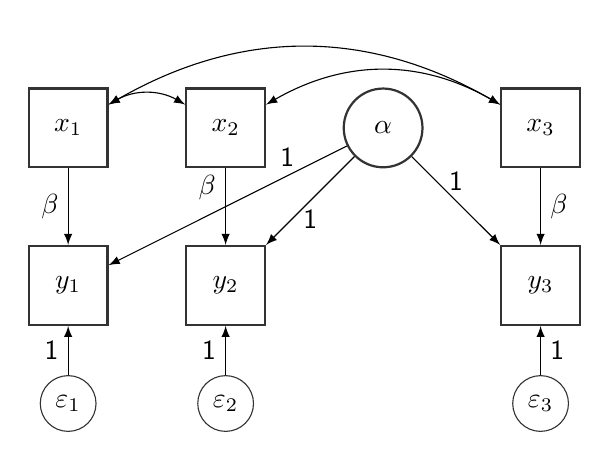
\begin{tikzpicture}
% Node styles ---
\tikzstyle{man} = [rectangle, thick, minimum size = 1cm, draw = black!80, fill = white!100, font = \sffamily] % Manifest variables
\tikzstyle{lat} = [circle, thick, minimum size = 1cm, draw = black!80, fill = white!100, font = \sffamily] % Latent variables
\tikzstyle{err} = [circle, draw = black!80, fill = white!100, font = \sffamily] % Errors 
% Edge styles
\tikzstyle{con} = [-latex, font = \sffamily] % Effects
\tikzstyle{cons} = [-latex, font = \sffamily\small] % Effects with smaller font 
\tikzstyle{cor} = [latex-latex, font = \sffamily] % Correlations
% Begin Figure ---
% Nodes 
\node at (+0.0,+0.0) [man] (x1) {$x_{1}$};
\node at (+2.0,+0.0) [man] (x2) {$x_{2}$};
\node at (+6.0,+0.0) [man] (x3) {$x_{3}$};
\node at (+4.0,+0.0) [lat] (eta) {$\alpha$};
\node at (+0.0,-2.0) [man] (y1) {$y_{1}$};
\node at (+2.0,-2.0) [man] (y2) {$y_{2}$};
\node at (+6.0,-2.0) [man] (y3) {$y_{3}$};
\node at (+0.0,-3.5) [err] (e1) {$\varepsilon_{1}$};
\node at (+2.0,-3.5) [err] (e2) {$\varepsilon_{2}$};
\node at (+6.0,-3.5) [err] (e3) {$\varepsilon_{3}$};
% Paths
\path (x1) edge [con, draw = black!100, left] node {$\beta$} (y1);
\path (x2) edge [con, draw = black!100, left, near start] node {$\beta$} (y2);
\path (x3) edge [con, draw = black!100, right] node {$\beta$} (y3);
\path (e1) edge [con, draw = black!100, left] node {1} (y1);
\path (e2) edge [con, draw = black!100, left] node {1} (y2);
\path (e3) edge [con, draw = black!100, right] node {1} (y3);
\path (eta) edge [con, draw = black!100, above, near start] node {1} (y1);
\path (eta) edge [con, draw = black!100, below] node {1} (y2);
\path (eta) edge [con, draw = black!100, above] node {1} (y3);
% correlations
\path (x1) edge [cor, bend left] node {} (x2);
%\path (x1) edge [cor, bend left] node {} (eta);
\path (x1) edge [cor, bend left] node {} (x3);
%\path (x2) edge [cor, bend left] node {} (eta);
\path (x2) edge [cor, bend left] node {} (x3);
%\path (x3) edge [cor, bend right] node {} (eta);
\end{tikzpicture}
}
\caption{Typical three-wave RE-SEM model with contemporary effects\label{fig:resem}}
\end{center}
\end{figure}

\begin{figure}
\begin{center}
\resizebox{0.75\textwidth}{!}{%
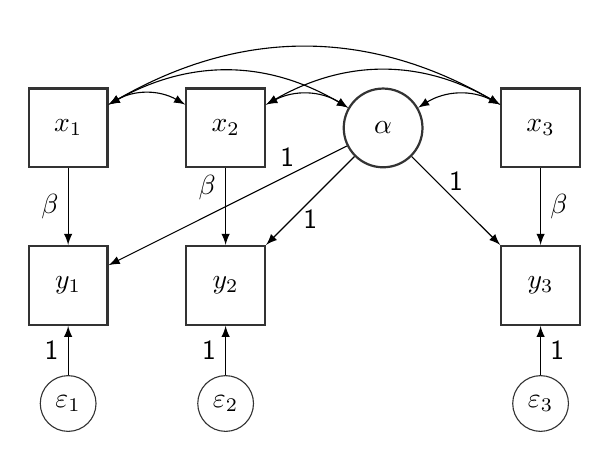
\begin{tikzpicture}
% Node styles ---
\tikzstyle{man} = [rectangle, thick, minimum size = 1cm, draw = black!80, fill = white!100, font = \sffamily] % Manifest variables
\tikzstyle{lat} = [circle, thick, minimum size = 1cm, draw = black!80, fill = white!100, font = \sffamily] % Latent variables
\tikzstyle{err} = [circle, draw = black!80, fill = white!100, font = \sffamily] % Errors 
% Edge styles
\tikzstyle{con} = [-latex, font = \sffamily] % Effects
\tikzstyle{cons} = [-latex, font = \sffamily\small] % Effects with smaller font 
\tikzstyle{cor} = [latex-latex, font = \sffamily] % Correlations
% Begin Figure ---
% Nodes 
\node at (+0.0,+0.0) [man] (x1) {$x_{1}$};
\node at (+2.0,+0.0) [man] (x2) {$x_{2}$};
\node at (+6.0,+0.0) [man] (x3) {$x_{3}$};
\node at (+4.0,+0.0) [lat] (eta) {$\alpha$};
\node at (+0.0,-2.0) [man] (y1) {$y_{1}$};
\node at (+2.0,-2.0) [man] (y2) {$y_{2}$};
\node at (+6.0,-2.0) [man] (y3) {$y_{3}$};
\node at (+0.0,-3.5) [err] (e1) {$\varepsilon_{1}$};
\node at (+2.0,-3.5) [err] (e2) {$\varepsilon_{2}$};
\node at (+6.0,-3.5) [err] (e3) {$\varepsilon_{3}$};
% Paths
\path (x1) edge [con, draw = black!100, left] node {$\beta$} (y1);
\path (x2) edge [con, draw = black!100, left, near start] node {$\beta$} (y2);
\path (x3) edge [con, draw = black!100, right] node {$\beta$} (y3);
\path (e1) edge [con, draw = black!100, left] node {1} (y1);
\path (e2) edge [con, draw = black!100, left] node {1} (y2);
\path (e3) edge [con, draw = black!100, right] node {1} (y3);
\path (eta) edge [con, draw = black!100, above, near start] node {1} (y1);
\path (eta) edge [con, draw = black!100, below] node {1} (y2);
\path (eta) edge [con, draw = black!100, above] node {1} (y3);
% correlations
\path (x1) edge [cor, bend left] node {} (x2);
\path (x1) edge [cor, bend left] node {} (eta);
\path (x1) edge [cor, bend left] node {} (x3);
\path (x2) edge [cor, bend left] node {} (eta);
\path (x2) edge [cor, bend left] node {} (x3);
\path (x3) edge [cor, bend right] node {} (eta);
\end{tikzpicture}
}
\caption{Typical three-wave FE-SEM model with contemporary effects\label{fig:fesem}}
\end{center}
\end{figure}

\hypertarget{fesem}{%
\section{Random and fixed effects in lavaan}\label{fesem}}

The basic panel models discussed in this tutorial consist of three main
parts. First, we want to create a latent variable representing the
individual effects. Second, we regress the time-varying dependent
variable on the time-varying (and time-invariant, see Section
\ref{time-invariant}) covariates. Third, we specify the correlations
depending on our assumptions. If we believe the individual effects are
unrelated to the time-varying covariates (we must assume they are
unrelated to the time-invariant ones, otherwise the model is not
identified), then we apply the RE assumptions and constrain the
covariances between the individual effects and the time-varying
covariates to zero. If we believe the individual effects are indeed
related to the model covariates (or more realistic assumption in many
circumstances), then we must specify these correlations between the
individual effects and the time-varying covariates. Finally, in an
optional step, we can constrain the residual variances to be equal over
time, if we want or need to, potentially in order to save degrees of
freedom. The following section will explain these steps in
\texttt{lavaan} in detail.

\hypertarget{the-lavaan-package-in-r}{%
\subsection{\texorpdfstring{The \texttt{lavaan} package in
\texttt{R}}{The lavaan package in R}}\label{the-lavaan-package-in-r}}

The package \texttt{lavaan} needs to be installed once with
\texttt{install.packages("lavaan")}. This can be entered directly into
the console or at the top of the script. To be able to use the package,
we need to load it for every new \texttt{R} session:

\singlespacing

\begin{Shaded}
\begin{Highlighting}[]
\KeywordTok{library}\NormalTok{( lavaan)}
\end{Highlighting}
\end{Shaded}

\doublespacing

For users unfamiliar with \texttt{R}, SEM analyses can be carried out
with almost no knowledge of the language. Typically, someone unfamiliar
with \texttt{R} would prepare their data using some other statistical
software, and then save the intended dataset as a \texttt{.csv},
\texttt{.xlsx}, \texttt{.dta}, \texttt{.sav}, etc. file. The user must
then import the data, preferably as a dataframe, and the rest occurs
using the \texttt{lavaan} syntax.\footnote{There are many online
  tutorials for importing data in various formats, see, for example some
  from
  \href{https://www.datacamp.com/community/tutorials/r-data-import-tutorial}{datacamp}
  or
  \href{https://www.statmethods.net/input/importingdata.html}{Quick-R},
  or any of the many posts on
  \href{https://stackoverflow.com/search?q=r+import+data}{stackoverflow}.}

To use \texttt{lavaan}, we create an \texttt{R} object using the
assignment operator \texttt{\textless{}-}, see the model syntax example
below. Here, the object has been called \texttt{fe\_sem} because the
option for the individual effects to covary with the time-varying
covariates has been chosen (more on that in a moment). The object can be
named anything that complies with object naming conventions in
\texttt{R} (e.g., the object name must start with a letter or dot,
separate using underscores or dots, etc.). The model syntax is enclosed
in quotes, either single \texttt{\textquotesingle{}\textquotesingle{}}
or double \texttt{""}. This means that the model syntax is essentially a
string that the \texttt{lavaan} package interprets in a second step.
Once the model has been specified, we use the \texttt{sem()} function to
`fit' the model. Notice a second object is made out of the fitted
\texttt{lavaan} object. Here the fitted \texttt{lavaan} object has been
named \texttt{fe\_sem.fit}. That is, we specify the SEM by writing the
model syntax as a string and saving it as an object. Then, in a second
step, we run the \texttt{sem()} function on that object. The
\texttt{sem()} function requires at least two arguments: \texttt{model},
i.e., the model object (here: \texttt{fe\_sem}), and \texttt{data},
i.e., the dataframe or covariance matrix (along with the mean vector, if
desired). That is, at a bare minimum, we must tell \texttt{lavaan} how
the model is specified and where the data is. There are a number of
other optional arguments that can be included. If they are not, the
defaults of the \texttt{sem()} wrapper are used.\footnote{See
  \href{https://rdrr.io/cran/lavaan/man/sem.html}{further details on the
  \texttt{sem()} wrapper defaults}, or enter \texttt{lavOptions()} into
  the console to get a full list of defaults. An explanation of the
  optional arguments can be found by entering \texttt{?lavOptions} in
  the console. There are other `wrappers' with slightly different
  default options, like \texttt{cfa()} for example, see
  \href{https://lavaan.ugent.be/tutorial/cfa.html}{the \texttt{lavaan}
  tutorial website}.} Many default options are uninteresting for the
current tutorial, but it is important to note that the \texttt{sem()}
wrapper allows all latent exogenous variables to covary,

For this example, even though it is the default estimator,
\texttt{estimator\ =\ "ML"} has been included as an optional argument to
emphasize the fact. The
\href{https://github.com/henrik-andersen/FE-SEM/blob/master/simulation-code.R}{online
supplementary materials} provide some guidance on using robust
estimators and full information maximum likelihood (FIML) to deal with
non-normal data and missing values; both of which can be accessed with
optional arguments in the \texttt{sem()} function call.

\hypertarget{model-syntax}{%
\subsection{Model syntax}\label{model-syntax}}

Again, specifying the most basic random or fixed effects model, like the
one shown in \citet{Bollen2010} (the same model as Equation
\eqref{eq:fe} but with just one time-varying predictor) involves three
to four components. First, we define the latent individual effects
variable using the \texttt{=\textasciitilde{}} `measured by' or
`manifested by' \citep{R-lavaan} operator at the same time constraining
the factor loadings at each timepoint to one with \texttt{1*} (see line
3 in the model code below). I will call the latent variable \texttt{a}
to stand for \(\alpha\). Constraining all of the factor loadings to one
reflects our implicit assumption that the combined effect of the
unit-specific unobserved factors is constant over time. This is the
default behaviour of traditional POLS-based approaches to RE and FE that
use the stacked long-format data.

Second, we regress the dependent variable on the independent variable
using the \texttt{\textasciitilde{}} regression operator (see lines
5--9). With stacked, long-format data, only one regression coefficient
is estimated over all observed timepoints. To have our model mimic this
behaviour, we need to constrain the the estimated coefficient to equal
over time. We do so by adding the same label to the regression
coefficient at every time point. We will use the label \texttt{b} (this
label was chosen arbitrarily, we could have used any letter or string of
characters) and have it act as an equality constraint for the regression
coefficient of interest \(\beta\).

The key to a FE model, as opposed to an RE model are our assumptions
about the relatedness of our time-varying covariates and the individual
effects, i.e., \(\mathop{\mathrm{\mathbb{E}}}[x_{t}\alpha]\). For an FE
model, we want to partial out any potential covariance between the
independent variable and the individual effects. This accounts for any
linear relationship between \(x_{t}\) and the unit-specific
characteristics influencing the dependent variable. Further, allowing
unrestricted covariances between the independent variable itself over
time will not affect how the coefficient \(\beta\) is estimated, but
will have an effect on the standard errors (see lines 12--17). To mimic
the behaviour of a conventional FE model, we allow the independent
variable to be correlated with the individual effects and itself over
time. Covariances (including covariances between a variable and itself,
i.e., variances) are specified using the
\texttt{\textasciitilde{}\textasciitilde{}} operator. The alternative RE
model is achieved by replacing line 11 with line 12, which is currently
commented out. In line 12, the covariances between the individual
effects and the time-varying covariate are constrained to zero; the RE
assumption. This is done in the same way as fixing the factor loadings
to one in line 3. Here, we fix the covariances to zero with \texttt{0*}.

The last component of our code involves the variances of the residuals
(lines 19--23). This component is optional, but we can constrain the
residual variances to be equal over time to again mimic the behaviour of
a conventional RE/FE model using POLS on stacked data. Here, again, we
use labels to make equality constraints. Because \(y_{t}\) is
endogenous, the \texttt{\textasciitilde{}\textasciitilde{}} operator
specifies the variances of \emph{residuals}, i.e., \(\varepsilon_{t}\).

\singlespacing

\doublespacing

\singlespacing

\begin{Shaded}
\begin{Highlighting}[numbers=left,,]
\NormalTok{fe\_sem \textless{}{-}}\StringTok{ \textquotesingle{}}
\StringTok{\# Define individual effects variable }
\StringTok{a =\textasciitilde{} 1*y1 + 1*y2 + 1*y3 + 1*y4 + 1*y5}
\StringTok{\# Regressions, constrain coefficient to be equal over time}
\StringTok{y1 \textasciitilde{} b*x1}
\StringTok{y2 \textasciitilde{} b*x2 }
\StringTok{y3 \textasciitilde{} b*x3}
\StringTok{y4 \textasciitilde{} b*x4}
\StringTok{y5 \textasciitilde{} b*x5}
\StringTok{\# Correlations, individual effects are related to time{-}varying }
\StringTok{\# covariates depending on RE or FE assumptions }
\StringTok{a \textasciitilde{}\textasciitilde{} x1 + x2 + x3 + x4 + x5             \# FE Model }
\StringTok{\# a \textasciitilde{}\textasciitilde{} 0*x1 + 0*x2 + 0*x3 + 0*x4 + 0*x5 \# RE Model }
\StringTok{x1 \textasciitilde{}\textasciitilde{} x2 + x3 + x4 + x5}
\StringTok{x2 \textasciitilde{}\textasciitilde{} x3 + x4 + x5}
\StringTok{x3 \textasciitilde{}\textasciitilde{} x4 + x5}
\StringTok{x4 \textasciitilde{}\textasciitilde{} x5}
\StringTok{\# Constrain residual variances to be equal over time}
\StringTok{y1 \textasciitilde{}\textasciitilde{} e*y1}
\StringTok{y2 \textasciitilde{}\textasciitilde{} e*y2}
\StringTok{y3 \textasciitilde{}\textasciitilde{} e*y3}
\StringTok{y4 \textasciitilde{}\textasciitilde{} e*y4}
\StringTok{y5 \textasciitilde{}\textasciitilde{} e*y5}
\StringTok{\textquotesingle{}}
\NormalTok{fe\_sem.fit \textless{}{-}}\StringTok{ }\KeywordTok{sem}\NormalTok{(}\DataTypeTok{model =}\NormalTok{ fe\_sem, }
                  \DataTypeTok{data =}\NormalTok{ dfw, }
                  \DataTypeTok{estimator =} \StringTok{"ML"}\NormalTok{)}
\end{Highlighting}
\end{Shaded}

\doublespacing

\hypertarget{ex1}{%
\section{A simulated example}\label{ex1}}

To demonstrate the application of FE models in SEM, a dataset can be
simulated that embodies the FE assumptions. Again, the code for data
simulation can be found in the
\href{https://github.com/henrik-andersen/FE-SEM/blob/master/simulation-code.R}{online
supplementary materials}.

To show that the latent individual effects variables represent the
\emph{combined} effect of all time-invariant characteristics, the
dependent variable will be influenced by two separate unit-specific
variables, which we can call \(\alpha_{1}\) and \(\alpha_{2}\). We will
construct the simulated data such that the independent variable is
correlated with both of the time-invariant variables. This means that
approaches that fail to account for this confounding influence, such as
POLS or RE, will be biased.

The wide-format equations for the data generating process can be
described as: \begin{align}
\bm{x_{t}} & = \bm{\alpha_{1}}\beta_{x_{t},\alpha_{1}} + \bm{\alpha_{2}}\beta_{x_{t},\alpha_{2}} + \bm{\delta_{t}}, \\
\bm{y_{t}} & = \bm{x_{t}}\beta_{y_{t},x_{t}} + \bm{\alpha_{1}}\beta_{y_{t},\alpha_{1}} + \bm{\alpha_{2}} \beta_{y_{t},\alpha_{2}} + \bm{\varepsilon_{t}} 
\end{align} where, for the sake of simplicity, \(\bm{\alpha_{1}}\),
\(\bm{\alpha_{2}}\), \(\bm{\delta_{t}}\) and \(\bm{\varepsilon_{t}}\)
are \(\sim N(0,1)\).

For the following example, a sample size of 1,000, observed over five
waves, was chosen. The unique variance of \(\bm{x}\), as well as both
the individual-effect variables is also \(\sim N(0,1)\). The coefficient
of interest, \(\beta_{y,x}\) is set to be equal to \(0.3\). A
correlation between \(\bm{x}\) and the individual effects is induced
through \(\beta_{x,\alpha_{1}} = 0.85\) and
\(\beta_{x,\alpha_{1}} = 0.50\). With the variances above set to one,
the covariances will be roughly
\(\mathop{\mathrm{\mathrm{Cov}}}(x_{t},\alpha_{1}) = 0.85\) and
\(\mathop{\mathrm{\mathrm{Cov}}}(x_{t},\alpha_{2}) = 0.5\). The
dependent variable is also influenced by the individual effects
variables with \(\beta_{y_{t},\alpha_{1}} = 0.75\) and
\(\beta_{y_{t},\alpha_{2}} = 0.45\) These values were chosen
arbitrarily.

\singlespacing

\doublespacing

We can get a summary of the model with \texttt{summary()}. The first
portion of the summary output gives an overview of some basic
information and fit statistics. The maximum likelihood estimator is the
default, so it did not have to be explicitly selected in the fitting
function call. Other estimators are available, including generalized and
unweighted least squares (\texttt{GLS} and \texttt{ULS}, respectively),
robust standard errors maximum likelihood (\texttt{MLM}) and several
others (see \href{https://lavaan.ugent.be/tutorial/est.html}{the lavaan
online tutorial for more}).

This part of the summary output also tells us that the analysis is based
on 1,000 observations (missings would be shown here as well if there
were any), and that the \(\chi^{2}\) statistic is 30.138 based on 32
degrees of freedom (55 observed covariances minus 1 error variance, 1
coefficient, 1 latent variable variance, 5 exogenous variable variances
and 15 covariances for \(55 - 23 = 32\) df). The p-value on the
\(\chi^{2}\) statistic is not significant with \(p =\) 0.561 which tells
us the differences between the model-implied and observed covariance
matrices are likely due to chance, and that the model fits the data well
(given how the data was generated, it would be surprising if this were
not the case). Other fit measures including typical comparative fit
indices can be requested by either adding \texttt{fit.measures\ =\ TRUE}
as a secondary argument to the \texttt{summary()} call, or by asking for
a complete list of all available fit statistics using
\texttt{lavInspect(model,\ "fit")} where \texttt{model} stands for the
name of the fitted model, in this case \texttt{fe\_sem.fit}.

\singlespacing

\begin{Shaded}
\begin{Highlighting}[]
\KeywordTok{summary}\NormalTok{(fe\_sem.fit)}
\end{Highlighting}
\end{Shaded}

\begin{verbatim}
## lavaan 0.6-7 ended normally after 37 iterations
## 
##   Estimator                                         ML
##   Optimization method                           NLMINB
##   Number of free parameters                         31
##   Number of equality constraints                     8
##                                                       
##   Number of observations                          1000
##                                                       
## Model Test User Model:
##                                                       
##   Test statistic                                30.138
##   Degrees of freedom                                32
##   P-value (Chi-square)                           0.561
## 
## Parameter Estimates:
## 
##   Standard errors                             Standard
##   Information                                 Expected
##   Information saturated (h1) model          Structured
...
\end{verbatim}

\doublespacing

Next the summary output shows the measurement models for the latent
variables, if any. In this case the latent variable \texttt{a} for
\(\alpha\) is measured by each of the five observed dependent variables
with factor loadings fixed to 1.0.

\singlespacing

\begin{verbatim}
...
## Latent Variables:
##                    Estimate  Std.Err  z-value  P(>|z|)
##   a =~                                                
##     y1                1.000                           
##     y2                1.000                           
##     y3                1.000                           
##     y4                1.000                           
##     y5                1.000                           
...
\end{verbatim}

\doublespacing

The regressions are shown next. Here, because we have constrained the
regression coefficients to be equal over time (the equality constraint
label \texttt{(b)} is listed to the left of the estimates), the estimate
of \(\beta =\) 0.294 (0.016) is repeated five times. The corresponding
z- and p-values show that the coefficient is, unsurprisingly,
significant.

\singlespacing

\begin{verbatim}
...
## Regressions:
##                    Estimate  Std.Err  z-value  P(>|z|)
##   y1 ~                                                
##     x1         (b)    0.294    0.016   18.809    0.000
##   y2 ~                                                
##     x2         (b)    0.294    0.016   18.809    0.000
##   y3 ~                                                
##     x3         (b)    0.294    0.016   18.809    0.000
##   y4 ~                                                
##     x4         (b)    0.294    0.016   18.809    0.000
##   y5 ~                                                
##     x5         (b)    0.294    0.016   18.809    0.000
...
\end{verbatim}

\doublespacing

Next, the covariance estimates are listed. First, the covariances
between the latent individual effects variable and the independent
variable over time are shown, and then the covariances between the
independent variable with itself over time.

One should always take care to double-check that there are no unintended
covariances listed here. Like \texttt{Mplus}, the \texttt{lavaan}
package estimates some covariances per default, without the user
explicitly having to add them to the model syntax. For example,
covariances between latent variables are estimated per default. If one
does not wish for them to covary, it must be explicitly stated, e.g.,
with \texttt{f1\ \textasciitilde{}\textasciitilde{}\ 0*f2}, assuming the
latent variables are called \texttt{f1} and \texttt{f2}, or by
overriding the default behaviour for the entire model by adding
\texttt{orthogonal\ =\ TRUE} (which sets the correlation between all
latent variables to zero) to the fitting call.\footnote{This is at least
  the current behaviour of both the \texttt{cfa} and \texttt{sem}
  wrappers. In fact, both wrappers seem to be identical in terms of the
  default settings, see \citet{Rosseel2020}.}

\singlespacing

\begin{verbatim}
...
## Covariances:
##                    Estimate  Std.Err  z-value  P(>|z|)
##   a ~~                                                
##     x1                0.844    0.055   15.355    0.000
##     x2                0.867    0.056   15.441    0.000
##     x3                0.845    0.055   15.400    0.000
##     x4                0.822    0.053   15.455    0.000
##     x5                0.820    0.053   15.572    0.000
##   x1 ~~                                               
##     x2                0.908    0.070   12.900    0.000
##     x3                0.935    0.069   13.466    0.000
##     x4                0.921    0.067   13.661    0.000
##     x5                0.914    0.067   13.716    0.000
##   x2 ~~                                               
##     x3                0.889    0.070   12.675    0.000
##     x4                0.922    0.069   13.423    0.000
##     x5                0.889    0.068   13.165    0.000
##   x3 ~~                                               
##     x4                0.865    0.067   12.976    0.000
##     x5                0.901    0.066   13.554    0.000
##   x4 ~~                                               
##     x5                0.850    0.064   13.285    0.000
...
\end{verbatim}

\doublespacing

Finally, the variance estimates are listed. Here, we see that in order
to mimic the behaviour of a traditional FE model, the error variances
over time were specified to be equal using the equality constraint
\texttt{(e)}. Notice the \texttt{.} beside \texttt{y1}, \texttt{y2},
etc.: this indicates that the listed variance refers to an endogenous
variable, and that it is thus an error variance. In this case, these
refer to the variances of \(\varepsilon_{t}\). After that, the variances
of the exogenous variables, both observed and unobserved are listed.

\singlespacing

\begin{verbatim}
...
## Variances:
##                    Estimate  Std.Err  z-value  P(>|z|)
##    .y1         (e)    1.022    0.023   44.721    0.000
##    .y2         (e)    1.022    0.023   44.721    0.000
##    .y3         (e)    1.022    0.023   44.721    0.000
##    .y4         (e)    1.022    0.023   44.721    0.000
##    .y5         (e)    1.022    0.023   44.721    0.000
##     x1                1.986    0.089   22.361    0.000
##     x2                2.079    0.093   22.361    0.000
##     x3                1.987    0.089   22.361    0.000
##     x4                1.860    0.083   22.361    0.000
##     x5                1.814    0.081   22.361    0.000
##     a                 0.799    0.052   15.310    0.000
\end{verbatim}

\doublespacing

\hypertarget{extensions}{%
\section{Extensions}\label{extensions}}

\hypertarget{relax}{%
\subsection{Relaxing assumptions meant to mimic traditional FE
models}\label{relax}}

There are a number of implicit assumptions attached to the typical FE
model that can be relaxed in SEM. Some of these assumptions have been
discussed already, and a fairly comprehenisve list of assumptions can be
found in \citet{Bollen2010}. Here, I will go over just a few,
concentrating on the implementation in \texttt{lavaan} and the
opportunity to empirically test whether the adjustments are justified or
not.

The assumptions we will discuss here pertain to the time-invariance of
the effects of both the latent individual effects and the observed
covariates, as well as a time-invariant error variance. We can also
empirically test the correlation between the individual effects and the
covariates to see whether a RE model is preferable to the FE model.

For example, we can rewrite the original FE equation as \begin{align}
y_{it} & = \beta_{t}x_{it} + \lambda_{t}\alpha_{i} + \varepsilon_{it}
\end{align} where \(\beta\) becomes \(\beta_{t}\) and the implicit
regression weight of one turns to \(\lambda_{t}\) to highlight the fact
that the effect of \(x\) as well as \(\alpha\) on \(y\) may vary over
time. We can furthermore easily relax the assumption of time-constant
error variance, i.e., \(\sigma^{2}_{\varepsilon_{t}}\). As noted in the
\href{https://github.com/henrik-andersen/FE-SEM/blob/master/article.pdf}{main
article}, the assumption regarding
\(\mathop{\mathrm{\mathbb{E}}}[\alpha x_{t}]\) in \(\bm{\Psi}\)
determines whether we have an FE or RE model. We can set these to zero
and test whether the RE model would be preferable to the FE model. In
general, if the individual effects are truly uncorrelated with the model
covariates, it is advisable to switch to an RE model since because it
uses up less degrees of freedom, it will have smaller standard errors
\citep{Bollen2010}.

In the following \texttt{lavaan} code, we simply remove the factor
loadings of one for the latent individual effect variable which allows
them to be estimated freely at each timepoint. For the effect of the
covariate, we can either delete the constraints \texttt{b} in
\texttt{yt\ \textasciitilde{}\ b*xt} or give each regression a different
label, e.g., \texttt{b1}, \texttt{b2}, \texttt{b3}, etc. Similarly, to
allow the error variance to vary over time, we turn the constraints
\texttt{e} into simple labels, i.e., \texttt{e1}, \texttt{e2},
\texttt{e3}, etc., or again just delete them. In fact, regarding the
error variances, they will be estimated necessarily, and do not need to
be explicitly mentioned in the model syntax at all. Finally, to move
from an FE to an RE model, we could simply constrain the correlations
between the individual effects and the covariates to zero, i.e.,
\texttt{a\ \textasciitilde{}\textasciitilde{}\ 0*x1\ +\ 0*x2\ +\ 0*x3\ +\ 0*x4\ +\ 0*x5}.

\singlespacing

\begin{Shaded}
\begin{Highlighting}[numbers=left,,]
\NormalTok{fe\_sem\_fullyrelaxed \textless{}{-}}\StringTok{ \textquotesingle{}}
\StringTok{\# Define individual effects variable }
\StringTok{a =\textasciitilde{} y1 + y2 + y3 + y4 + y5}
\StringTok{\# Regressions, constrain coefficient to be equal over time}
\StringTok{y1 \textasciitilde{} b1*x1}
\StringTok{y2 \textasciitilde{} b2*x2 }
\StringTok{y3 \textasciitilde{} b3*x3}
\StringTok{y4 \textasciitilde{} b4*x4}
\StringTok{y5 \textasciitilde{} b5*x5}
\StringTok{\# Allow unrestricted correlation between eta and covariates}
\StringTok{a \textasciitilde{}\textasciitilde{} x1 + x2 + x3 + x4 + x5}
\StringTok{\# Alternatively: constrain all to 0 for RE model, or}
\StringTok{\# just individual correlations}
\StringTok{\# a \textasciitilde{}\textasciitilde{} 0*x1 + 0*x2 + 0*x3 + 0*x4 + 0*x5}
\StringTok{x1 \textasciitilde{}\textasciitilde{} x2 + x3 + x4 + x5}
\StringTok{x2 \textasciitilde{}\textasciitilde{} x3 + x4 + x5}
\StringTok{x3 \textasciitilde{}\textasciitilde{} x4 + x5}
\StringTok{x4 \textasciitilde{}\textasciitilde{} x5}
\StringTok{\# Constrain residual variances to be equal over time}
\StringTok{y1 \textasciitilde{}\textasciitilde{} e1*y1}
\StringTok{y2 \textasciitilde{}\textasciitilde{} e2*y2}
\StringTok{y3 \textasciitilde{}\textasciitilde{} e3*y3}
\StringTok{y4 \textasciitilde{}\textasciitilde{} e4*y4}
\StringTok{y5 \textasciitilde{}\textasciitilde{} e5*y5}
\StringTok{\textquotesingle{}}
\NormalTok{fe\_sem\_fullyrelaxed.fit \textless{}{-}}\StringTok{ }\KeywordTok{sem}\NormalTok{( }\DataTypeTok{model =}\NormalTok{ fe\_sem\_fullyrelaxed, }
                                \DataTypeTok{data =}\NormalTok{ dfw, }
                                \DataTypeTok{estimator =} \StringTok{"ML"}\NormalTok{)}
\end{Highlighting}
\end{Shaded}

\doublespacing

\singlespacing

\doublespacing

As outlined in \citet{Bollen2010}, the researcher has the opportunity to
test each of the assumptions empirically and decide whether a more
parsimonious, i.e., restrictive model is justifiable. For each
assumption, a likelihood ratio test can be carried out to determine
whether the improvement to model fit resulting from the relaxation of
various assumptions is significant or whether the more parsimonious
model is preferable after all.

If we use the original model \texttt{fe\_sem.fit} (from the
\href{https://github.com/henrik-andersen/FE-SEM/blob/master/article.pdf}{main
article}) as a starting point, the best strategy for testing these
assumptions is to work in a stepwise fashion, relaxing one assumption at
a time. We can begin by first constraining the correlation between
\(\alpha\) and \(x_{t}\) to zero (\texttt{re\_sem}) for an RE model. If
turning from an FE to an RE model does not significantly worsen model
fit, we can go forward with the rest of the steps with the RE model. If,
however, the fit does worsen significantly, it is likely better to stick
with the FE model; moving forward then with it to see if a less
restrictive FE model is preferable. We can perform a likelihood ratio
test in \texttt{R} using the \texttt{anova()} function:

\small
\singlespacing

\begin{Shaded}
\begin{Highlighting}[]
\KeywordTok{anova}\NormalTok{( fe\_sem.fit, re\_sem.fit)}
\end{Highlighting}
\end{Shaded}

\begin{verbatim}
## Chi-Squared Difference Test
## 
##            Df   AIC   BIC   Chisq Chisq diff Df diff Pr(>Chisq)    
## fe_sem.fit 32 30998 31111  30.137                                  
## re_sem.fit 37 31809 31897 850.928     820.79       5  < 2.2e-16 ***
## ---
## Signif. codes:  0 '***' 0.001 '**' 0.01 '*' 0.05 '.' 0.1 ' ' 1
\end{verbatim}

\doublespacing
\normalsize

The table that is generated shows a comparison of the nested models, in
decending order according to degrees of freedom. The RE model does not
estimate the correlations between the individual effects and the
covariates, so it is more parsimonious and thus listed at the bottom.
The \texttt{Chisq} column shows the \(\chi^{2}\) statistic for both
models and the \texttt{Chisq\ diff} column calculates the difference
between the two. Obviously, according to the DGP, the correlation
between the individual effects and \(x_{t}\) is not zero, so fixing
these to zero leads to a substantial amount of misfit. The last column
puts the \(\chi^{2}\) difference in relation to the difference in
degrees of freedom and gives a p-value for the probability that the
difference is solely due to chance. Here, the change in \(\chi^{2}\) is
highly significant, so the FE model should be retained.

After now having established, based on the likelihood ratio test, that
FE is our preferred model, we can begin relaxing the rest of the
assumptions. I show the following merely as a demonstration of the
procedure, we know already from the DGP that the parsimonious model as
specified in \texttt{fe\_sem.fit} is appropriate. We can next allow the
error variances (\texttt{fe\_semb.fit}), the effect of \(x\) on \(y\)
(\texttt{fe\_semc.fit}) and finally the factor loadings of the
individual effects (\texttt{fe\_semd.fit}) all to vary over time.

\singlespacing

\doublespacing

\small
\singlespacing

\begin{Shaded}
\begin{Highlighting}[]
\KeywordTok{anova}\NormalTok{( fe\_sem.fit, fe\_semb.fit, fe\_semc.fit, fe\_semd.fit)}
\end{Highlighting}
\end{Shaded}

\begin{verbatim}
## Chi-Squared Difference Test
## 
##             Df   AIC   BIC  Chisq Chisq diff Df diff Pr(>Chisq)
## fe_semd.fit 20 31017 31189 25.140                              
## fe_semc.fit 24 31010 31162 25.764     0.6249       4     0.9603
## fe_semb.fit 28 31003 31135 26.686     0.9215       4     0.9215
## fe_sem.fit  32 30998 31111 30.137     3.4516       4     0.4853
\end{verbatim}

\doublespacing
\normalsize

Keep in mind that a less parsimonious model (fewer degrees of freedom)
can never fit worse than a more parsimonious one (more degrees of
freedom). I.e., chance variations due to sampling error mean that adding
constraints to a model will tend to always worsen fit, at least
minimally. The question here is whether the improvement to fit by
loosening constraints is meaningful or not. In the table above, we
should not expect any meaningful improvements moving from
\texttt{fe\_sem.fit} to \texttt{fe\_semd.fit}. Here, using simulated
data, we have the luxury of knowing that any significant differences in
\(\chi^{2}\) are due to chance. With real data, it is up to the
researcher to apply their best judgment and decide whether the results
are plausible or not.

\hypertarget{time-invariant}{%
\subsection{Time-invariant predictors}\label{time-invariant}}

What if we do not just want to just control for the effects of all
time-invariant variables, but investigate some of them in detail? Many
time-invariant variables, like sex, birth cohort, nationality,
education, etc. can be interesting on their own. And typically, many of
these variables are readily available in a given dataset. The
traditional OLS-based FE model does not allow for this, as it wipes out
the effect of \emph{all} time-invariant variables, whether observed or
not.

In SEM, we can easily specify a type of \emph{hybrid} FE/RE model
\citep{Bollen2010} that allows us to control for time-invariant
unobserved heterogeneity while also investigating the effects of
specific observed time-invariant predictors.\footnote{These types of
  models have become well known outside of SEM as well, see for example
  \citet{Allison2011}; \citet{Schunck2013}; \citet{Bell2018}.}

In the next example, we continue with the most complex model we have
specified so far, \texttt{fe\_sem4.fit} in which measurement error in
both the independent and dependent variables is accounted for using
latent variables. Now, we would like as well to specifically investigate
the effect of \(\alpha_{2}\) on the dependent variable. The equation for
this model changes to:
\(\eta_{t} = \beta \xi_{t} + \alpha + \gamma \alpha_{2} + \zeta_{t}\).

\singlespacing

\begin{Shaded}
\begin{Highlighting}[numbers=left,,]
\NormalTok{fe\_sem5 \textless{}{-}}\StringTok{ \textquotesingle{}}
\StringTok{\# Measurement model for dependent variable, n for eta}
\StringTok{n1 =\textasciitilde{} 1*y11 + y21 + y31}
\StringTok{n2 =\textasciitilde{} 1*y12 + y22 + y32}
\StringTok{n3 =\textasciitilde{} 1*y13 + y23 + y33}
\StringTok{n4 =\textasciitilde{} 1*y14 + y24 + y34}
\StringTok{n5 =\textasciitilde{} 1*y15 + y25 + y35}
\StringTok{\# Define individual effects variable }
\StringTok{a =\textasciitilde{} 1*n1 + 1*n2 + 1*n3 + 1*n4 + 1*n5}
\StringTok{\# Measurement model for independent variables, xi }
\StringTok{xi1 =\textasciitilde{} 1*x11 + x21 + x31 }
\StringTok{xi2 =\textasciitilde{} 1*x12 + x22 + x32}
\StringTok{xi3 =\textasciitilde{} 1*x13 + x23 + x33}
\StringTok{xi4 =\textasciitilde{} 1*x14 + x24 + x34}
\StringTok{xi5 =\textasciitilde{} 1*x15 + x25 + x35}
\StringTok{\# Regressions, constrain coefficient to be equal over time}
\StringTok{n1 \textasciitilde{} b*xi1 + g*a2}
\StringTok{n2 \textasciitilde{} b*xi2 + g*a2}
\StringTok{n3 \textasciitilde{} b*xi3 + g*a2}
\StringTok{n4 \textasciitilde{} b*xi4 + g*a2}
\StringTok{n5 \textasciitilde{} b*xi5 + g*a2}
\StringTok{\# Allow unrestricted correlation between eta and covariates}
\StringTok{a \textasciitilde{}\textasciitilde{} xi1 + xi2 + xi3 + xi4 + xi5 + 0*a2}
\StringTok{a2 \textasciitilde{}\textasciitilde{} xi1 + xi2 + xi3 + xi4 + xi5}
\StringTok{xi1 \textasciitilde{}\textasciitilde{} xi2 + xi3 + xi4 + xi5}
\StringTok{xi2 \textasciitilde{}\textasciitilde{} xi3 + xi4 + xi5}
\StringTok{xi3 \textasciitilde{}\textasciitilde{} xi4 + xi5}
\StringTok{xi4 \textasciitilde{}\textasciitilde{} xi5}
\StringTok{\# Constrain residual variances to be equal over time}
\StringTok{n1 \textasciitilde{}\textasciitilde{} e*n1}
\StringTok{n2 \textasciitilde{}\textasciitilde{} e*n2}
\StringTok{n3 \textasciitilde{}\textasciitilde{} e*n3}
\StringTok{n4 \textasciitilde{}\textasciitilde{} e*n4}
\StringTok{n5 \textasciitilde{}\textasciitilde{} e*n5}
\StringTok{\textquotesingle{}}
\NormalTok{fe\_sem5.fit \textless{}{-}}\StringTok{ }\KeywordTok{sem}\NormalTok{( }\DataTypeTok{model =}\NormalTok{ fe\_sem5, }
                    \DataTypeTok{data =}\NormalTok{ dfw, }
                    \DataTypeTok{estimator =} \StringTok{"ML"}\NormalTok{)}
\end{Highlighting}
\end{Shaded}

\doublespacing

Keep in mind, based on the DGP, the true parameters are \(\beta = 0.3\)
and \(\gamma = 0.45\).

\singlespacing

\begin{Shaded}
\begin{Highlighting}[]
\KeywordTok{summary}\NormalTok{(fe\_sem5.fit)}
\end{Highlighting}
\end{Shaded}

\begin{verbatim}
...
## Regressions:
##                    Estimate  Std.Err  z-value  P(>|z|)
##   n1 ~                                                
##     xi1        (b)    0.265    0.023   11.515    0.000
##     a2         (g)    0.490    0.033   14.999    0.000
##   n2 ~                                                
##     xi2        (b)    0.265    0.023   11.515    0.000
##     a2         (g)    0.490    0.033   14.999    0.000
##   n3 ~                                                
##     xi3        (b)    0.265    0.023   11.515    0.000
##     a2         (g)    0.490    0.033   14.999    0.000
##   n4 ~                                                
##     xi4        (b)    0.265    0.023   11.515    0.000
##     a2         (g)    0.490    0.033   14.999    0.000
##   n5 ~                                                
##     xi5        (b)    0.265    0.023   11.515    0.000
##     a2         (g)    0.490    0.033   14.999    0.000
...
\end{verbatim}

\doublespacing

From this we can see that such a hybrid model is does a good job of
estimating the coefficients of interest, with \(\hat{\beta} =\) 0.265
(0.023) and \(\hat{\gamma} =\) 0.49 (0.033).

It is important, however, to realize that the unbiasedness of
\(\hat{\gamma}\) in this model is dependent on the assumption that
\(\mathop{\mathrm{\mathbb{E}}}[\zeta | \bm{\xi_{t}}, \alpha_{2}] = 0\).
In other words, the idiosyncratic error is mean independent of
\(\bm{\xi_{t}} = (\xi_{1}, \xi_{2}, ..., \xi_{T})\) as well as
\(\alpha_{2}\). The first part is easier to accept because we are
controlling for all potential time-invariant confounders that could
induce a relationship between the independent variable and the error.
The unbiasedness of \(\hat{\gamma}\), on the other hand rests on the
assumption that the time-invariant predictor is independent of the
error. If \(\alpha_{2}\) represented the respondent's intelligence and
\(\eta_{t}\), the dependent variable, represented the respondent's
income, for example, then \(\hat{\gamma}\) would be biased if both were
dependent on a third time-invariant variable, say level of schooling, if
it is not controlled for. For this reason, we need to treat the
regression on a time-invariant predictor like any other regular
multivariate regression model and look to include all plausible
potential confounders as controls in the model, or turn to other
methods, e.g., instrumental variables.

\hypertarget{conclusion}{%
\section{Conclusion}\label{conclusion}}

Fixed effects regression in SEM has been outlined in well-known articles
by \citep{Allison2011, Bollen2010, Teachman2001}. This article provides
a focused look at the implementation of the basic model using the
\texttt{lavaan} package in \texttt{R}. The
\href{https://github.com/henrik-andersen/FE-SEM/blob/master/extensions.pdf}{online
supplementary materials} further discuss common extensions and some
tools for evaluating and loosening model assumptions.

The benefits of FE-SEM as opposed to traditional OLS-based FE-models are
largely the same ones that apply to the SEM framework in general: for
one, SEM allows for a great deal of flexibility. For example, it is easy
to loosen model constraints as necessary. Measurement error in both the
dependent and independent variables can be dealt with using latent
variables to achieve unbiased and more efficient results. Researchers
interested in time-invariant predictors can integrate them into a hybrid
FE/RE model with ease. Further extensions, like measurement invariance
testing \citep{Schoot2012, Millsap2011, Steenkamp1998} as well as lagged
dependent variables \citep{Bollen2010, Allison2017} for example, can
also be implemented in a straightforward fashion.

The most basic FE-SEM is furthermore the basis for a variety of
currently popular extended models, such as Latent Curve Models in
general \citep{Curran2001, Bollen2004}, as well as special
implementations like the Dynamic Panel Model \citep{Allison2017}, the
Random-Intercept Cross-Lagged Panel Model \citep{Hamaker2015} and the
Latent Curve Model with Structured Residuals \citep{Curran2014}. For
this reason it is all the more important for researchers to have a good
grasp on the method of applying panel regression in SEM, and
understanding the intuition of controlling for time-invariant
confounders. This article is meant to serve as a consolidated resource
for researchers looking for concrete advise on specifying FE and more
general panel models in SEM.

\bibliographystyle{tfcad}
\bibliography{references2.bib}




\end{document}
